\section{Robottens højde}
\label{sec:RHeight}
%

I denne section analyseres resultaterne med udgangspunkt i de forskellige højder robotten havde i testen. For hver af de 5 højder som blev anvendt, er der 7-10 besvarelser. De forskellige højder som blev anvendt i undersøgelsen er vist i \autoref{tab:RHeight}. Det undersøges hvordan robottens højde påvirker de rejsendes oplevelse af robotten, ved at undersøge hvordan resultaterne ændrer sig på tværs af de fem forskellige højder. Det er between subject design, da hver person kun har oplevet robotten i en af højderne og svaret ud fra denne.

% Det undersøges om robottens højde har en effekt på oplevelsen af robotten, ved hjælp af en principal component analysis.

\begin{table}[H]
\centering
\begin{tabular}{|l|l|}
\hline
Højde & Antal \\ \hline
118   & 9     \\ \hline
123.5 & 10    \\ \hline
129   & 9     \\ \hline
140   & 7     \\ \hline
151   & 8     \\ \hline
\end{tabular}
\caption{}
\label{tab:RHeight}
\end{table}

Ud fra scree plottet på \autoref{fig:RHeight-Scree} kan det ses at cirka 80 \& af variansen kan forklares ud fra de to første principal components. Ved at tage PC3 med, opnåes cirka 94 \% forklaret varians. Det er dog væsentligt simplere at fortolke resultaterne i to dimensioner og der kigges derfor som udgangspunkt kun på to primære komponenter.



\begin{figure}[H]
\centering
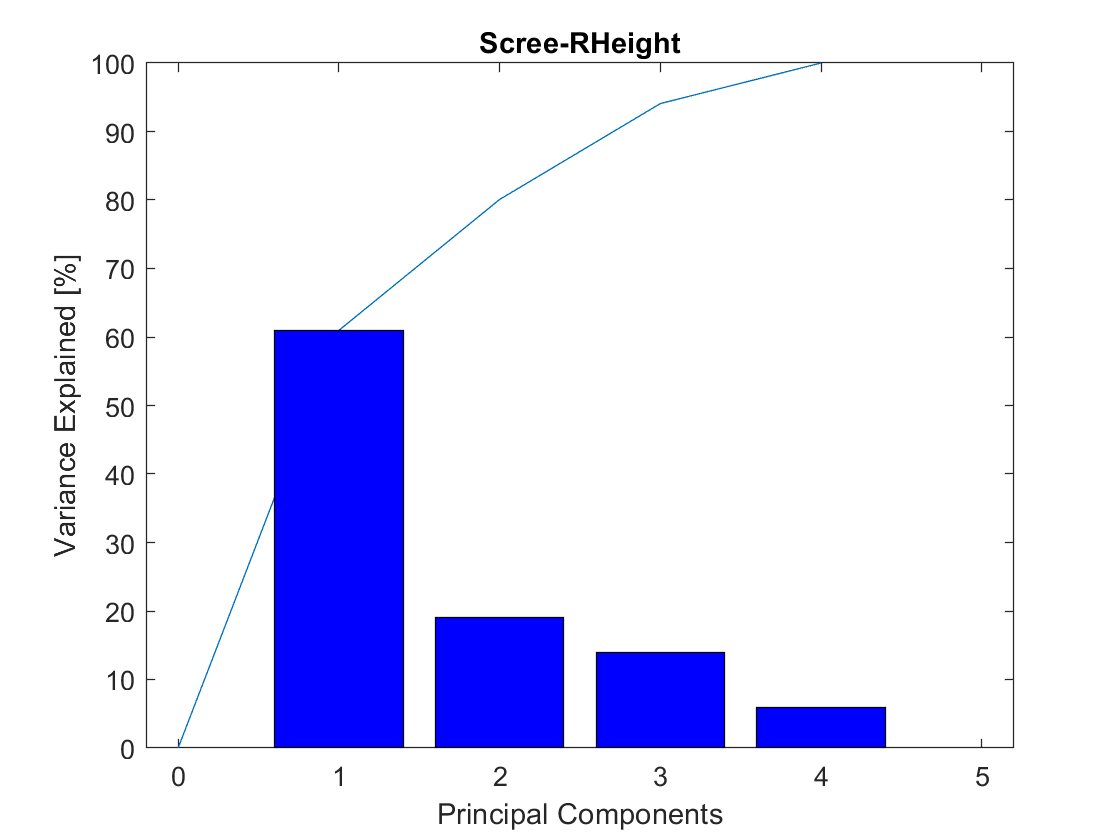
\includegraphics[width=\textwidth]{Figure/DatabehandlingSkalaer/PCAfigures/RHeight-Scree.png}
\caption{xx}
\label{fig:RHeight-Scree}
\end{figure}

Ud fra score-plottet på \autoref{fig:RHeight-Score} kan det ses at der generelt er en del spredning mellem resultaterne ud fra de fem forskellige højder, men at 129 og 140 har lignende karakteristikker, da de ligger meget tæt i plottet.

\begin{figure}[H]
\centering
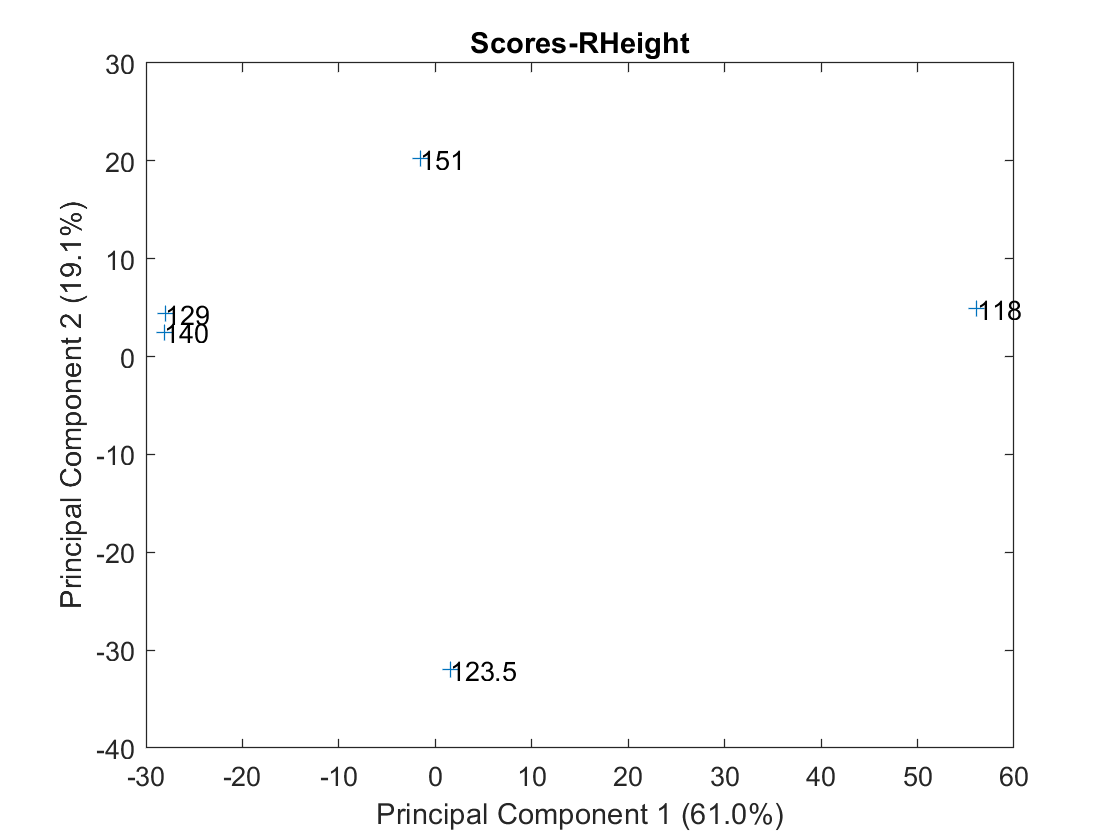
\includegraphics[width=\textwidth]{Figure/DatabehandlingSkalaer/PCAfigures/RHeight-Scores}
\caption{xx}
\label{fig:RHeight-Score}
\end{figure}
Ud fra biplottet på \autoref{fig:RHeight-biplot} kan det ses at Q19 bidrager mest til PC1, Q1 bidrager mest til PC2 og at 5,7,11 og 14 forklarer en meget lille del af variansen. 2 og 4 følges ad og ser ud til i høj grad at beskrive samme... noget med korrelation. Det samme gælder 12+18 og 8+17. Det giver ikke mening at snakke om de korte som følges ad, siden deres effekt er så lille at den ikke rigtigt bidrager til modellen. 
negativ korrelation mellem 21 og 18-12. 9 og 2+4. 16 og 19. Tjek om de her negative korrelationer giver mening
118 ligger i modsatte end af PC1 i forhold til 129+140. Hvilke parametre er det der får dem til at adskille sig på den mest forklarende akse? 123.5+151 adskiller sig på samme måde på PC2.

\begin{figure}[H]
\centering
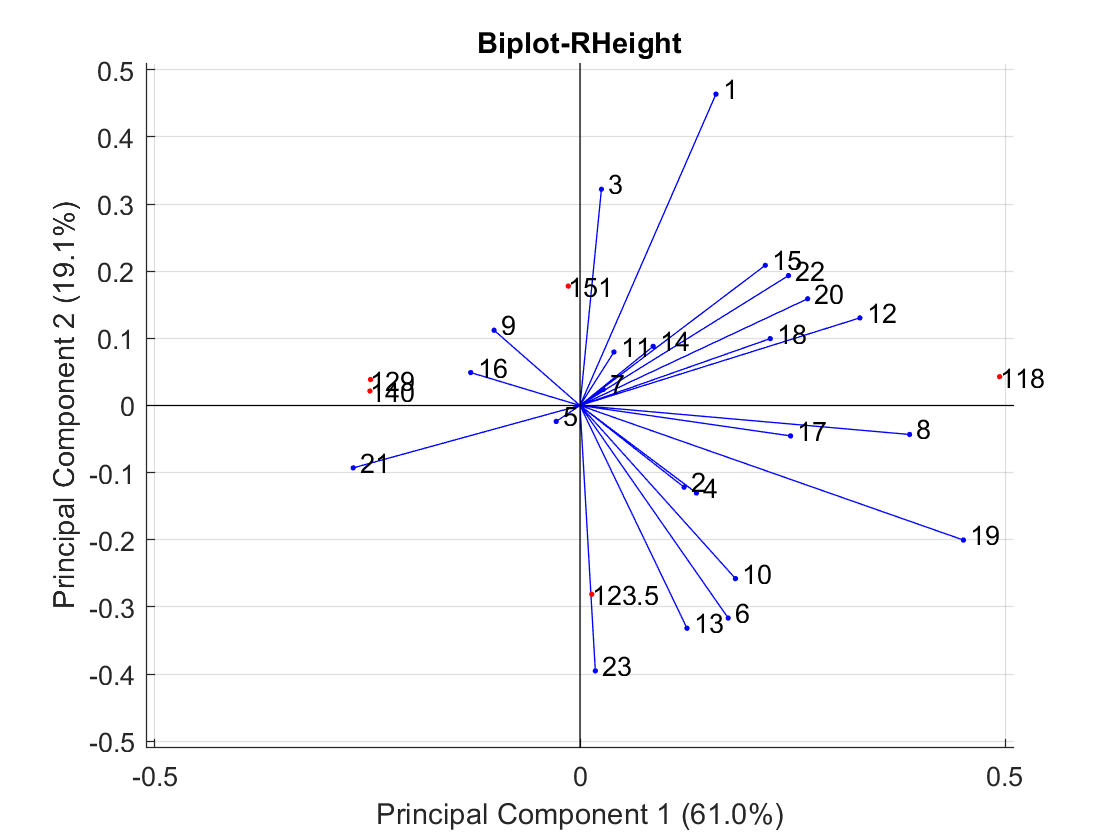
\includegraphics[width=\textwidth]{Figure/DatabehandlingSkalaer/PCAfigures/RHeight-Biplot.png}
\caption{xx}
\label{fig:RHeight-Biplot}
\end{figure}
 Ud fra loadings i tabel XX kan det ses at ... bidrager til...

S



Når man derimod kigger på 129 og 140 i et tredimensionelt biplot, se \autoref{fig:RHeight-3D}, kan det ses at de faktisk adskiller sig en del i den tredje dimension. 
6 og 10 bidrager mest til PC3.

Når man også tager den tredje PC med i plottet, forsvinder mange af ovenstående effekter, da de adskiller sig meget i den tredje dimension. 14, 15 og 22 ligger dog stadig relativt tæt og kan derfor muligvis være redundante. dækker over samme områder
\begin{figure}[H]
\centering
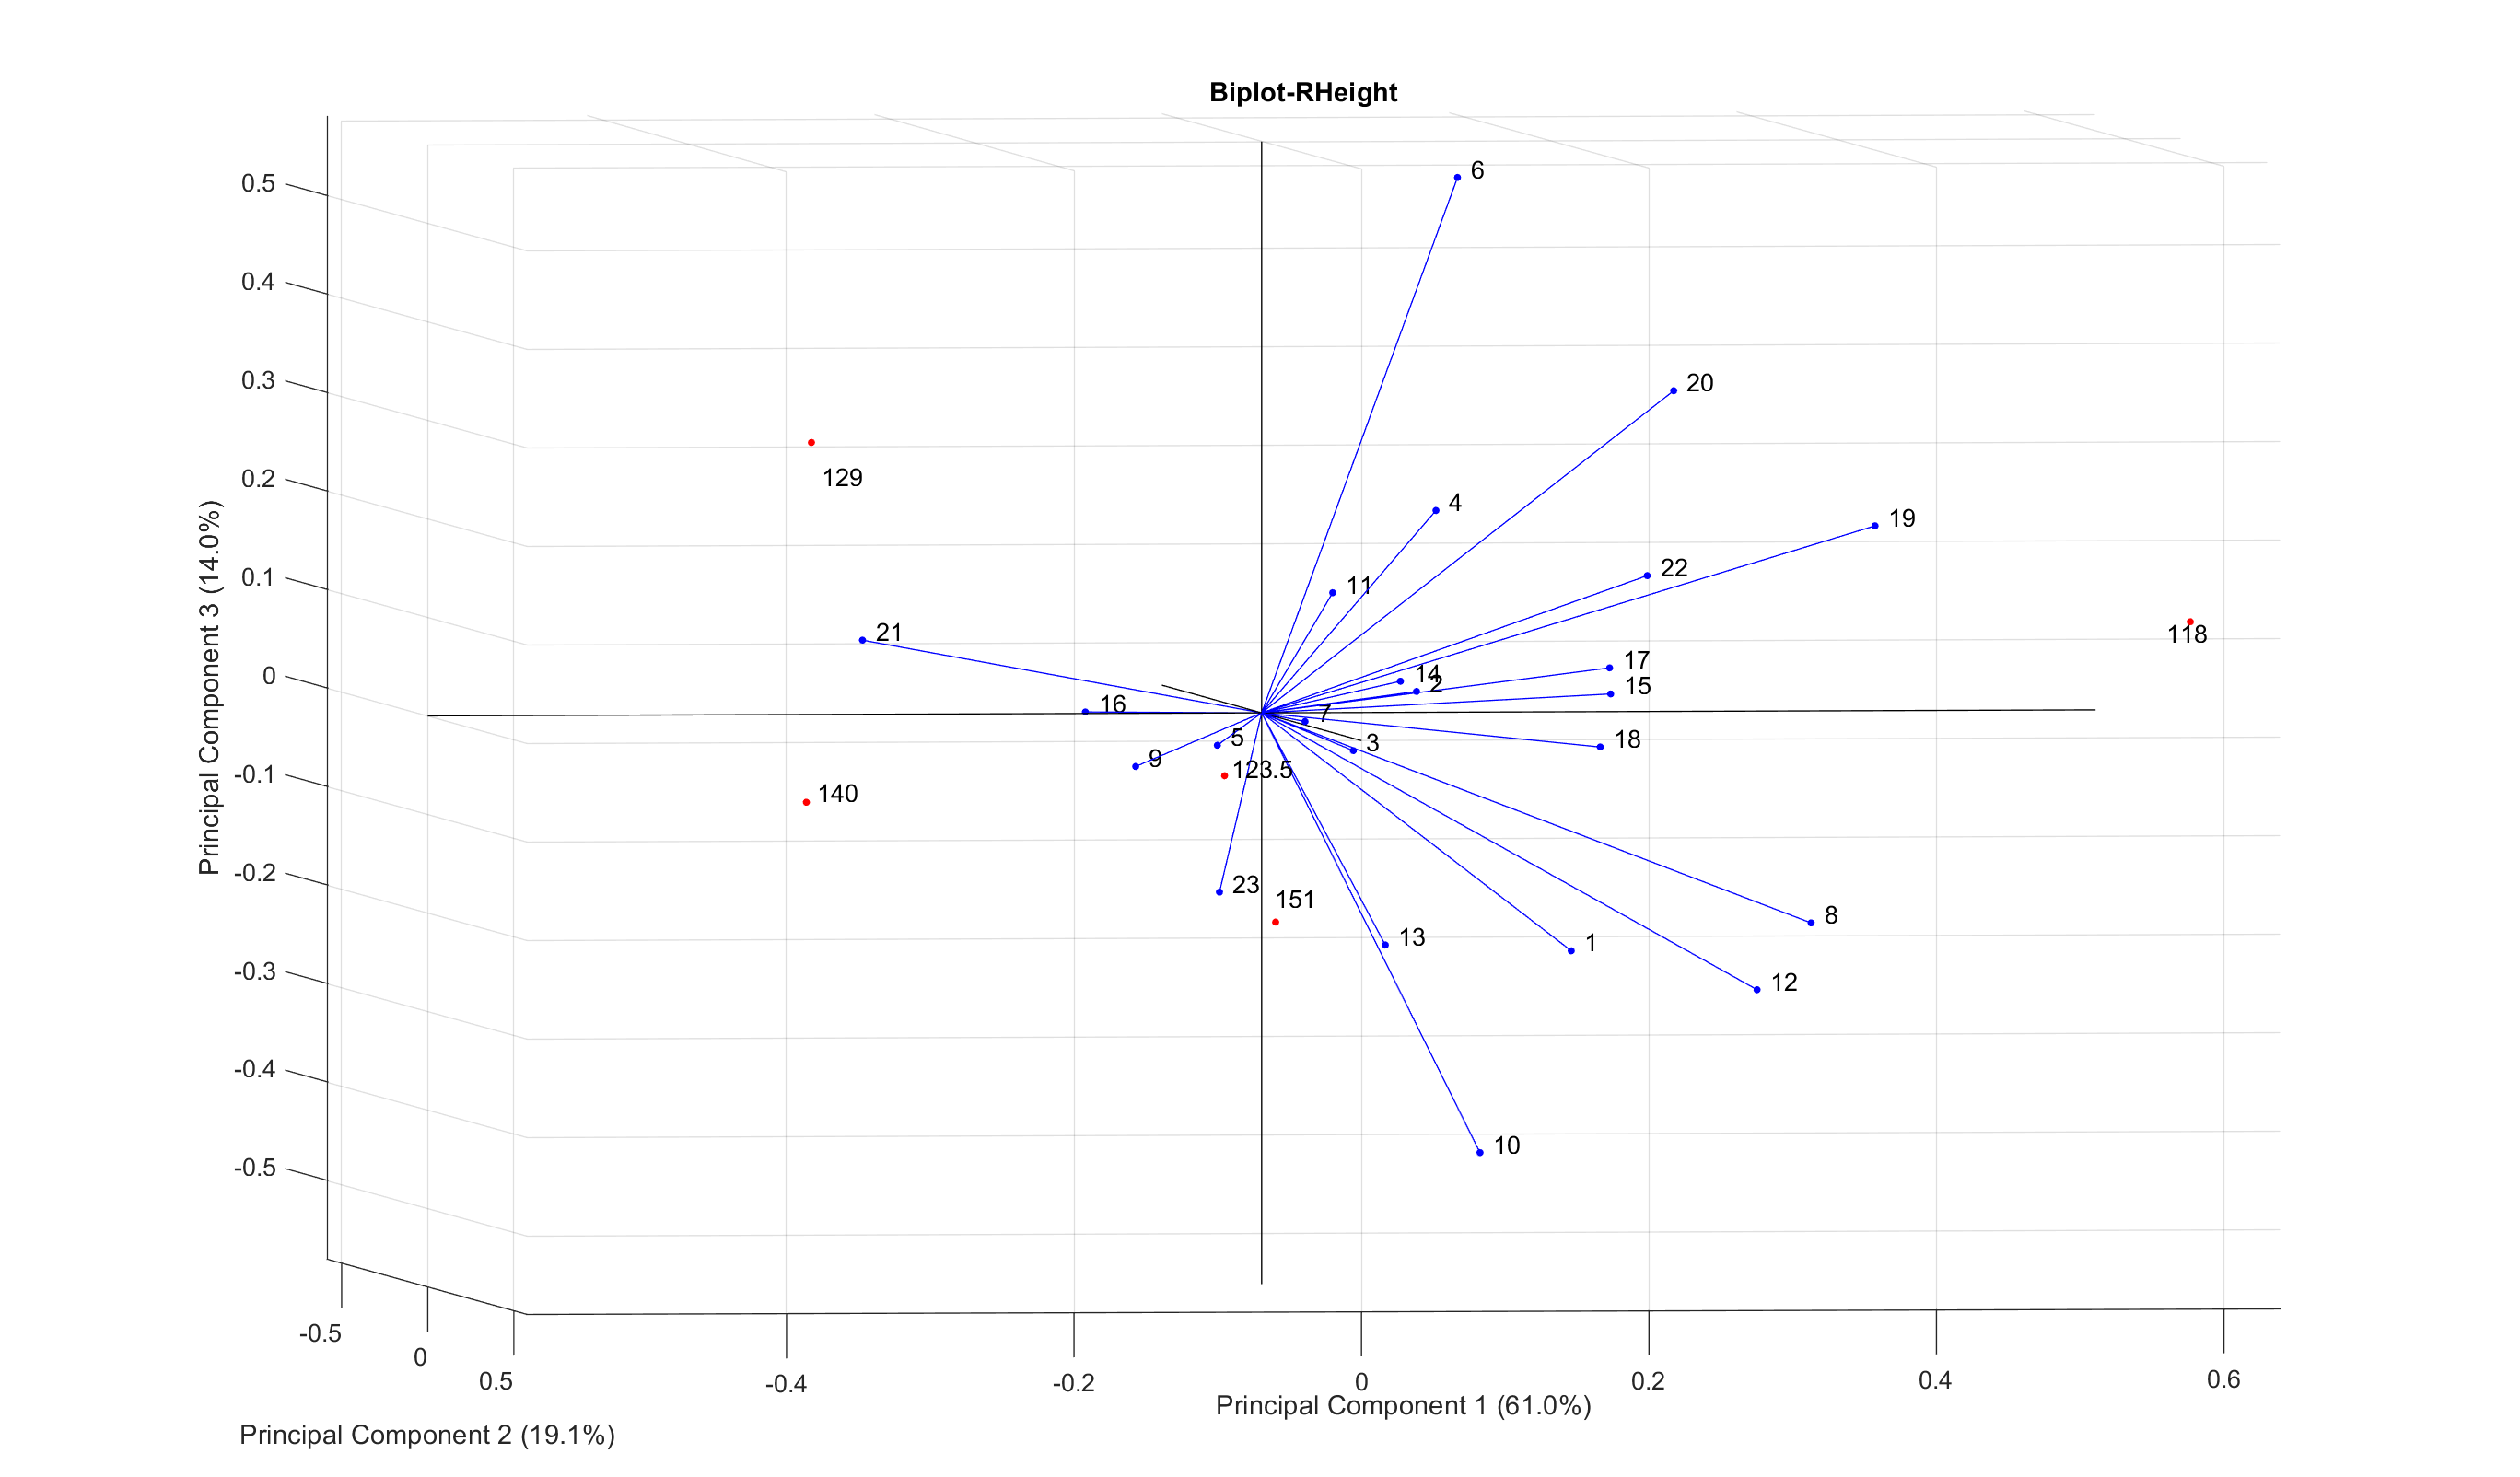
\includegraphics[width=\textwidth]{Figure/DatabehandlingSkalaer/PCAfigures/RHeight-3D.png}
\caption{xx}
\label{fig:RHeight-3D}
\end{figure}